\chapter{Funktion der Software}

\section{Verschlüsselungen}
\subsection{Die Wahl der Verschlüsselung}
Im Paper \cite{Doettling2021} wird kein Verschlüsselungsverfahren genannt. Jedes additiv homomorphe Verschlüsselungsverfahren kann theoretisch genutzt werden. Es werden jedoch einige Vorschläge  gemacht. Einer dieser Vorschläge ist das Paillier-Kryptosystem. Das Damgard-Jurik System, für das ich mich entschieden habe, ist eine Verallgemeinerung des Paillier-Kryptosystems. Unter anderem ist die Damgard-Jurik Verschlüsselung besser für Berechnungen mit mehreren Beteiligten geeignet, denn es gibt auch eine Threshold-Variante dieses Verschlüsselungs-Systems. \cite{IvanDamgard2004}
Ich habe mich bei der Verschlüsselung für das Damgard-Jurik Cryptosystem entschieden, weil es gut zu den Anforderungen, die wir haben, passt. Es ist speziell für den Anwendungsfall mit mehreren Parteien entworfen und ist deshalb auch in unserem Fall effizient.\\



\subsection{Damgard-Jurik Verschlüsselung}
Indem wir Shamirs Secret Sharing benutzen, können wir einen public Key und eine beliebige Anzahl an Private Key-Shares erstellen. Shamirs Secret Sharing basiert auf Polynominterpolation und kann beispielsweise auch genutzt werden, um dem System später noch neue Parteien hinzuzufügen.\cite{Shamir1979}\\
Durch die Nutzung der Damgard-Jurik Verschlüsselung kann jeder, der den public Key besitzt, Daten verschlüsseln. Entschlüsseln von Daten ist jedoch komplexer. Um Daten zu entschlüsseln, müssen genügend Parteien mit Private Key-Shares die Daten teilweise entschlüsseln. Danach müssen die partiellen Entschlüsselungen kombiniert werden. Hat man aber weniger als die benötigte Anzahl an partiellen Entschlüsselungen, werden keine Informationen sichtbar. \cite{IvanDamgard2004}\\
Einer der Hauptgründe, wegen dem ich mich für die Damgard-Jurik-Verschlüsselung entschieden habe ist, das man zum Entschlüsseln von Daten den Private Key nicht wiederherstellen muss. Dadurch kann der Schlüssel nicht missbraucht werden, um auch andere Dinge zu entschlüsseln. Dadurch müssen die Parteien keiner anderen Partei trauen und die Parteien können entscheiden, was entschlüsselt werden soll und was nicht. \cite{IvanDamgard2004}\\
Die Verschlüsselung erfüllt natürlich auch die andere große Anforderung, die wir haben. Die Verschlüsselung ist additiv homomorph, was wir für die Funktionalität des Protokolls brauchen. \cite{IvanDamgard2004}

\subsection{Übertragung der Python Implementierung}
Für die Implementierung der Verschlüsselung habe ich mich an der Python Implementierung \cite{swansonk14} orientiert. Da die Sicherheit der Verschlüsselung auf mathematischen Annahmen basiert  \cite{10.1007/3-540-48910-X_16}, muss mit großen Zahlen (mehr als 32 Bits) gerechnet werden, um sicher gegen Brute-Force-Angriffe zu sein. Daher entstehen bei der Übertragung der Python Implementierung nach Java einige Probleme. Da in Python Ganzzahlen beliebig groß werden können, aber in Java Ganzzahlen auf 32 Bit begrenzt sind, muss ich auf BigInteger zurückgreifen, um verschlüsselte Zahlen korrekt darstellen zu können.
Ein ähnliches Problem ist beispielsweise das Erstellen von zufälligen Primzahlen von bestimmter Länge. In Python stellt das kein Problem dar, aber in Java ist das erstellen von beliebig langen Primzahlen komplizierter. Trotz dieser Probleme habe ich eine funktionierende Implementierung der Damgard-Jurik Verschlüsslung geschaffen, die ich dann nutzen kann, um die Implementierung der komplexeren Teil-Protokolle zu testen.


\section{Architektur}
\section{Ring Realisierung}
Da in vielen der Unterprotokollen (OLS, ODT, secMult, secRank, secInv, SUR) Berechnungen über endlichen Körpern stattfinden, um Korrektheit und Sicherheit zu gewährleisten, benötigen wir eine robuste und effiziente Möglichkeit, mit endlichen Körpern zu arbeiten.\\
Da wir unter anderem lineare Gleichungssysteme über endlichen Körpern lösen müssen, und es nur wenige Java-Bibliotheken gibt, die diese Funktionalität anbieten, ist die Open-Source Bibliothek JLinalg \cite{JLinAlg} gut für unseren Fall geeignet. Die Bibliothek bietet aber standardmäßig nur eingeschränkte Funktionalitäten für beliebige Körper an. Das Lösen von linearen Gleichungssystemen ist eines der Dinge, die aber nur in den  Rationalen Zahlen oder dem Körper \{0;1\} möglich sind. Daher war es augenscheinlich am einfachsten, die Bibliothek zu erweitern, indem ich eine neue Klasse erstellt habe, wodurch die Bibliothek jetzt auch andere Funktionalitäten über beliebig großen Körpern berechnen kann. Unter anderem kann so auch das lineare Gleichungssystem gelöst werden.\\

\begin{lstlisting}[caption = Ausschnitt aus Teil-Protokoll secDT]
        private FModular(BigInteger val)
        {
            value = val.mod(modulus);
        }

        public static FModularFactory FACTORY(BigInteger i) {
            modulus = i;
            return FACTORY;
        }
        @Override
        public FModular add(FModular val)
        {
            return new FModular(value.add(val.value).mod(modulus));
        }
        
        
        @Override
        public FModular subtract(FModular val)
        {
            return new FModular((value.subtract(val.value)).mod(modulus));
        }

        @Override
        public FModular multiply(FModular val)
        {
            return new FModular(value.multiply(val.value).mod(modulus));
        }
        
        @Override
        public FModular divide(FModular val)
        {
            return new FModular(value.multiply(val.value.modInverse(modulus)).mod(modulus));
        }
\end{lstlisting}


\section{sichere Matrix Berechnungen}
Das grundlegendste Teil-Protokoll, das im Paper \cite{Doettling2021} vorgestellt wird, ist das secMult Protokoll, das genutzt werden kann, um verschlüsselte Matrizen, also Matrizen mit verschlüsselten Einträgen miteinander zu multiplizieren. Das ist ein wichtiger Bestandteil des Protokolls, denn diese Funktion wird in vielen Teil-Protokollen genutzt.\\
\begin{lstlisting}[caption = Ausschnitt aus dem secRank Teil-Protokoll \cite{Doettling2021}][firstnumber=3]
        All parties mutually compute Enc(pk, N) = Enc(pk, XUML) via three invocations of FOMM.
\end{lstlisting}
Interessanterweise lassen sich dadurch auch verschlüsselte Zahlen multiplizieren, indem Matrizen mit nur einem Eintrag erstellt werden und diese dann multipliziert werden. Dadurch, dass wir nun verschlüsselte Zahlen addieren können (durch die additiv homomorphe Verschlüsselung) und wir jetzt auch verschlüsselte Zahlen multiplizieren können, erreichen wir ähnliche Funktionalität, wie bei voll-homomorpher Verschlüsselung. Um Zahlen zu multiplizieren, brauchen wir zwar die Mithilfe der anderen Parteien, aber nicht das Vertrauen der anderen Parteien. Denn die anderen Parteien müssen zwar ihren Teil des Secret-Keys benutzen, um ihren Teil zur Matrix Multiplikation beizutragen, aber durch das gewählte Verschlüsselungsverfahren müssen sie weder ihren Secret-Key-Share verschicken, noch werden Informationen über ihren Secret-Key-Share bekannt.\\
Durch die nun praktisch voll-homomorphe Verschlüsselung bekommen wir viele mathematische Möglichkeiten, die wir in den anderen Teil-Protokollen nutzen können.
Ein Beispiel für die entstandenen Möglichkeiten ist die Polynommultiplikation im Teil-Protokoll secDT \cite{Doettling2021}.

\begin{figure}[h]
\begin{center}
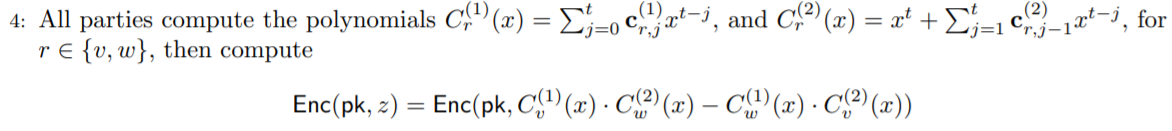
\includegraphics[width = 15cm]{secDTPart.png}
\caption{Ausschnitt aus Teil-Protokoll secDT}
\cite{Doettling2021}
\label{secDT}
\end{center}

\end{figure}

Um die verschlüsselten Polynome Cv(1) und Cw(2) miteinander zu multiplizieren, müssen wir verschlüsselte Zahlen miteinander multiplizieren. Wir können das Problem zwar teilweise umgehen, indem wir die verschlüsselten Polynome erst auswerten, wofür wir noch keine Multiplikation von verschlüsselten Zahlen nutzen müssen. In diesem Fall müssen wir aber danach die Ergebnisse der Auswertungen multiplizieren. In jedem Fall ist die Berechnung nur durch die erweiterte Funktionalität möglich.



